The aim of this chapter is to test and analyze projects from git by using developed module for RefactorErl. The projects selected for the experiment are written in Erlang and have more than 40 commits.

\section{Iron}

This project is functional Erlang Toolkit. Iron is released under the MIT license. It can do the foolowing:
\begin{itemize}
	\item Count with coerce equality, count with custom predicate.
	\item Find with coerce equality, find with custom predicate.
\end{itemize}

This project has just only one source code file with 68 commits.

We can see that with the version number increase the line of code number and char of code number also grow on Figure \ref{fig:loc_iron} and on Figure \ref{fig:char_iron}.

\begin{figure}[h]
	\centering
	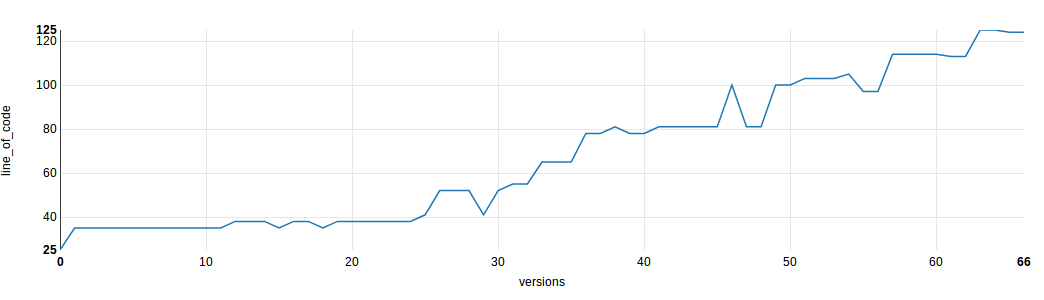
\includegraphics[height=45mm]{figures/loc_iron.png}
	\caption{Effective Line of code for fe.erl file.}
	\label{fig:loc_iron}
\end{figure}

\begin{figure}[h]
	\centering
	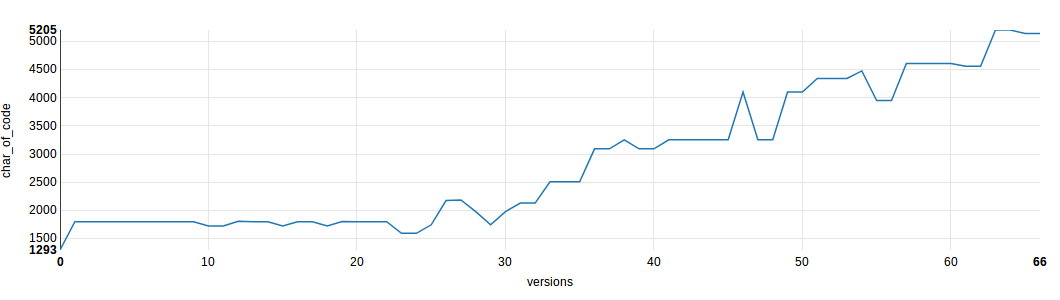
\includegraphics[height=45mm]{figures/char_iron.png}
	\caption{Char of code for fe.erl file.}
	\label{fig:char_iron}
\end{figure}

As shown on Figure \ref{fig:otp_iron} developer started to use otp library after 45th version. 

\begin{figure}[h]
	\centering
	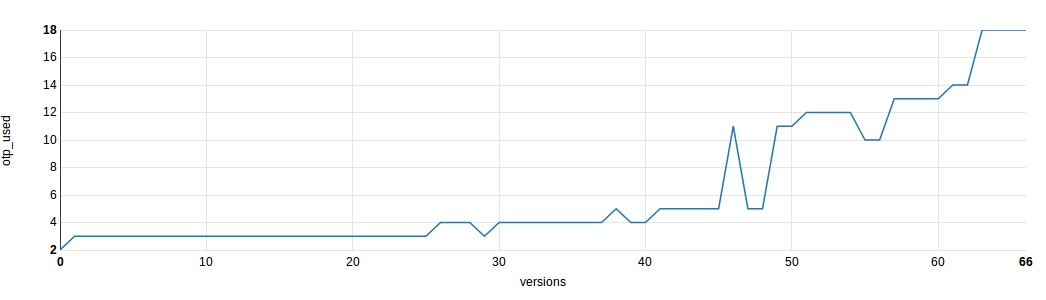
\includegraphics[height=45mm]{figures/otp_iron.png}
	\caption{Otp used for fe.erl file.}
	\label{fig:otp_iron}
\end{figure}

Average length of line was not stabilize until arround 35th version with gradually decreasing from 50 symbols to 38 symbols.

\begin{figure}[h]
	\centering
	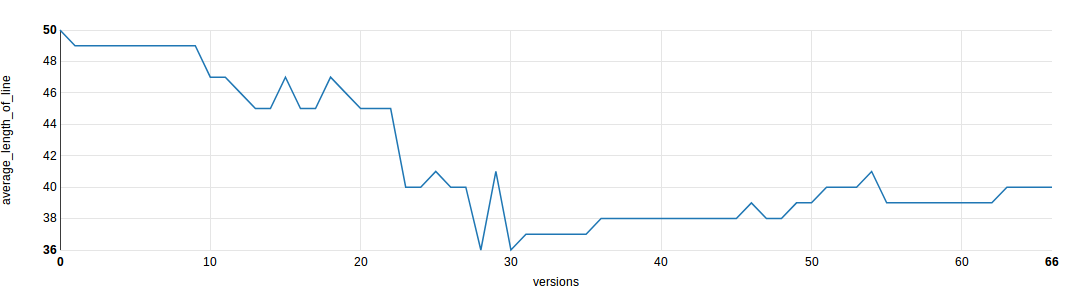
\includegraphics[height=45mm]{figures/average_length_of_line_iron.png}
	\caption{Average length of line for fe.erl file.}
	\label{fig:average_length_of_line_iron}
\end{figure}

As we can see on Figure \ref{fig:number_of_macros_iron} and Figure \ref{fig:number_of_records_iron} there are not defined macros and record in the whole iron project.

\begin{figure}[h]
	\centering
	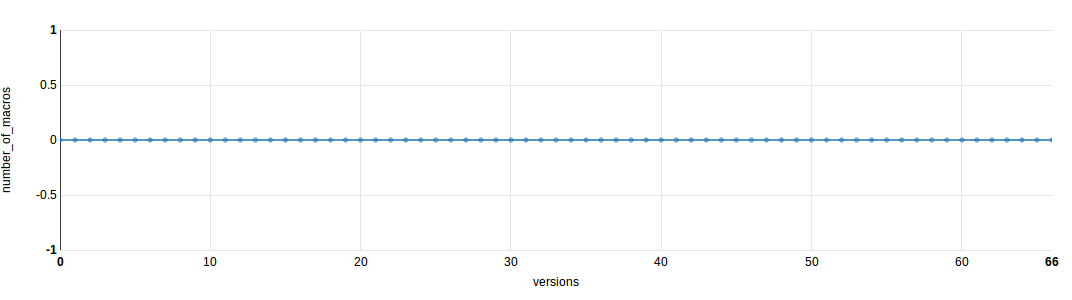
\includegraphics[height=45mm]{figures/number_of_macros_iron.png}
	\caption{Number of macros for fe.erl file.}
	\label{fig:number_of_macros_iron}
\end{figure}

\begin{figure}[h]
	\centering
	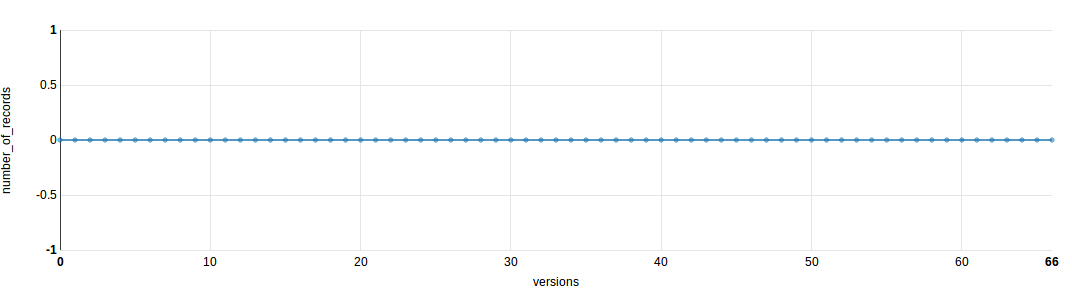
\includegraphics[height=45mm]{figures/number_of_records_iron.png}
	\caption{Number of records for fe.erl file.}
	\label{fig:number_of_records_iron}
\end{figure}

\section{Erlang chat }

This project is multi user chat written in Erlang. It has nine source code files and 45 commits.
